One of the most important tasks of a DBMS is to figure out an efficient \textbf{evaluation plan} (also termed \textbf{execution plan} or \textbf{access plan}) for high level statements \\

Query processing is a 3-step process:
\begin{enumerate}
    \item Parsing and translation (from SQL to RA)
    \item Optimization (refine RA expression)
    \item Evaluation (exec Ra operators)
\end{enumerate}

\subsection{Query Processing}
\textbf{Query cost} is generally measured as the \textbf{total elapsed time} for answering a query. Many factors contribute to time cost, but typically \textbf{disk access is the predominant cost}. The cost of disk access is measured by taking into account:
\begin{itemize}[label=\(\rhd\)]
    \item Number of seeks * average-seek-cost
    \item Number of blocks read * average-block-read-cost
    \item Number of blocks written * average-block-write-cost
        \begin{itemize}[label=\(\rhd\)]
            \item Cost to wirte a block is greater than cost to read, since data is read back after being written
        \end{itemize}
        \item For simplicity, just use \textbf{number of block transfers from disk} as the cost measure
\end{itemize}

\subsubsection{Sorting, Partitioning}

If relation fits in memory, use techniques like \textbf{quicksort}, else use external sorting, like \textbf{external sort-merge}.\\

\noindent
\textbf{\underline{External Sort-Merge}}\\

\begin{itemize}[label=\(\rhd\)]
    \item \textbf{Step 1: Create N sorted runs} (M is \# blocks in buffer)
    \begin{enumerate}
        \item Let $i$ be 0 initially 
        \item Repeatedly do the following until the end of the relation
        \begin{enumerate}[label*=\arabic*.]
            \item Read $M$ blocks of the relation (or the rest) into memory
            \item Sort the in-memory blocks
            \item Write sorted data to run file $R_i$
            \item Increment $i$
        \end{enumerate}
    \end{enumerate}
    \item \textbf{Step 2: Merge runs (N-way merge)} (assume $N<M$)
    \item[] (Use $N$ blocks in memory to buffer input runs, and 1 block to buffer output)
    \begin{enumerate}
        \item Read the first block of each run $R_i$ into its buffer page
        \item \textbf{Repeat until} all input buffer pages are empty
        \begin{enumerate}[label*=\arabic*.]
            \item Select the first record (in sort order) among all buffer pages
            \item Write the record to the output buffer. If the output buffer is full write it to disk 
            \item Delete the record from its input buffer page
            \item \textbf{If} the buffer page becomes empty \textbf{then}
            \begin{itemize}[label=\(\rhd\)]
                \item[] read the next block (if any) of the run into buffer
            \end{itemize}
        \end{enumerate}
    \end{enumerate}
    \item If $N \geq M$, \textbf{several merge passes} (step 2) are required
    \begin{itemize}[label=\(\rhd\)]
        \item In each pass, contiguous groups of $M-1$ runs are merged
    \end{itemize}
\end{itemize}
\begin{figure}[H]
    \centering
    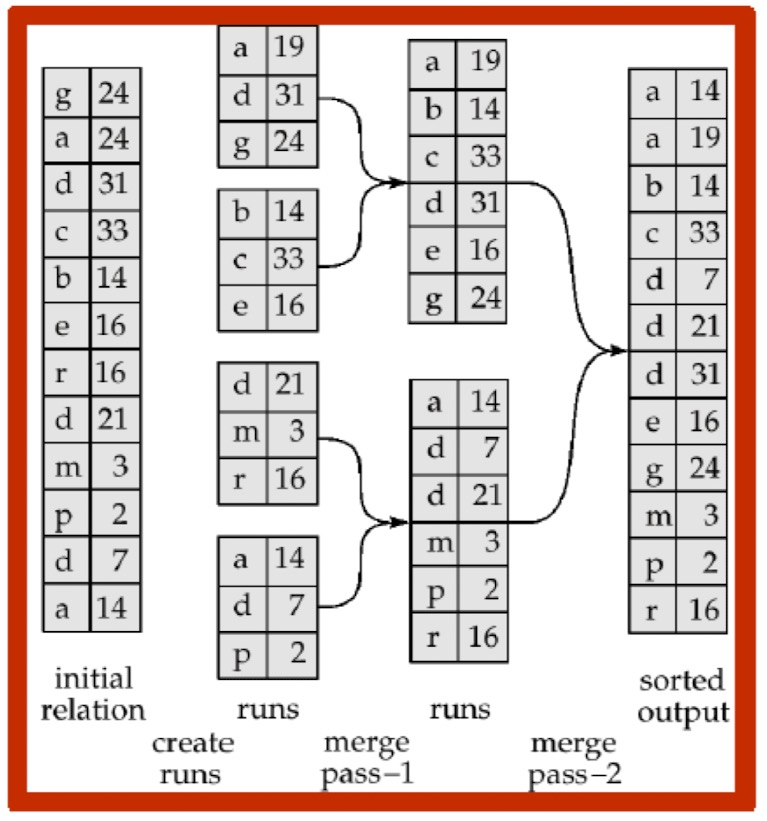
\includegraphics[width=0.5\linewidth]{images/Screenshot 2024-05-25 at 11.58.54.jpg}
    \caption{External Merge Sort (M=3, 1 block = 1 tuple)}
\end{figure}
\begin{itemize}[label=\(\rhd\)]
    \item \textbf{Cost analysis}
    \begin{itemize}[label=\(\rhd\)]
        \item $b_r=$ number of blocks in $r$
        \item Initial number of runs: $\lceil b_r/M\rceil$
        \item Total number of merge passes required: $\lceil \log _{M-1}(b_r/M)\rceil$
        \begin{itemize}[label=\(\rhd\)]
            \item The number of runs decreases by a factor of $M-1$ in each merge pass
        \end{itemize}
        \item Disk accesses for initial run creation and in each pass is $2b_r$
        \begin{itemize}[label=\(\rhd\)]
            \item Exception: For final pass there is no write cost 
        \end{itemize}
        \item Thus total number of disk accesses for external sorting:\[
        Cost=b_r(2 \lceil \log_{M-1} (\lceil b_r/M\rceil ) \rceil +1)
        \]
    \end{itemize}
\end{itemize}


\subsubsection{Selection Evaluation Strategies}

The strategy/algorithm for the evaluation of the selection operator depends 
\begin{itemize}[label=\(\rhd\)]
    \item on the type of the selection condition
    \item on the available index structures
\end{itemize}

Types of selection conditions:
\begin{itemize}[label=\(\rhd\)]
    \item \textbf{Equality queries}: $\sigma_{a=v}(r)$
    \item \textbf{Range queries}: $\sigma_{a\leq v}(r) $ or $\sigma_{a\geq v}(r) $
    \begin{itemize}[label=\(\rhd\)]
        \item Can be implemented by using:
        \begin{itemize}[label=\(\rhd\)]
            \item Linear File Scan
            \item Binary Search
            \item Index Scan
        \end{itemize}
    \end{itemize}
    \item \textbf{Conjunctive selection}: $\sigma_{\theta_1 \land \theta_2 \land \cdots \land \theta_n}(r)$
    \item \textbf{Disjunctive selection}: $\sigma_{\theta_1 \lor \theta_2 \lor \cdots \lor \theta_n}(r)$
\end{itemize}


Evaluation Strategies: 
\begin{itemize}[label=\(\rhd\)]
    \item \textbf{A1 Linear search}: Scan each file block and test all records to see whether they satisfy the selection condition
    \begin{itemize}[label=\(\rhd\)]
        \item Fairly expensive, but always applicable
        \item Cost estimate ($b_r$ = number of blocks in file):
        \begin{itemize}[label=\(\rhd\)]
            \item Worst case: $Cost = b_r$
            \item If the selection is on a key attribute: $Average\ cost = b_r/2$ (stop when finding record)
        \end{itemize}
    \end{itemize}
    \item \textbf{A2 Binary Search}: Apply binary search to locate records that satisfy selection condition
    \begin{itemize}[label=\(\rhd\)]
        \item Only applicable if relation already sorted, and selection condition is on the attribute that the file is ordered on
            \item Cost estimate for $\sigma_{A=v}(r)$: 
        \begin{itemize}[label=\(\rhd\)]
        \item $\lceil \log_2(b_r) \rceil $ = cost of locating the first tuple by binary search on the blocks 
        \item Plus number of blocks containing records that satisfy selection condition
        \end{itemize}
    \end{itemize}
    \item \textbf{A3 Primary Index + equality on candidate key}
    \begin{itemize}[label=\(\rhd\)]
        \item Retrieve a single record that satisfies the equality condition
        \item $Cost = \underbrace{HT_i}_\text{search in index} + \underbrace{1}_\text{get data}$(height of B+ tree + 1 data block)
    \end{itemize}
    \item \textbf{A4 Primary index + equality on non-candidate key}
    \begin{itemize}[label=\(\rhd\)]
        \item Retrieve multiple records, where records are on consecutive blocks
        \item $Cost=HT_i+ \# $ blocks with records with given search key
    \end{itemize}
    \item \textbf{A5 Secondary index + equality on search-key} 
    \begin{itemize}[label=\(\rhd\)]
        \item Retrieve a single record if the search-key is a candidate key
        \begin{itemize}[label=\(\rhd\)]
            \item $Cost=HT_i+1$
        \end{itemize}
        \item Retrieve multiple records is search-key is not a candidate key
        \begin{itemize}[label=\(\rhd\)]
            \item $Cost = HT_i + \#$buckets with search-key value + $\#$ retrieved records
            \item Can be very expensive, since each record may be on a different block
            \item Linear file scan may be cheaper if many records have to be fetched
        \end{itemize}
    \end{itemize}
    \item \textbf{A6 Primary index on A + non-equality condition}
    \begin{itemize}[label=\(\rhd\)]
        \item $\sigma_{A\geq v}$: Use index to find first tuple $\geq v$; then scan relation sequentially
        \item $\sigma_{A\leq v}$: Scan relation sequentially until first tuple $>v$; do not use index
    \end{itemize}
    \item \textbf{A7 Secondary index on A + non-equality condition}
    \begin{itemize}[label=\(\rhd\)]
        \item $\sigma_{A\geq v}$: Use index to find first index entry $\geq v$; scan index sequentially from there, to find pointers to records
        \item $\sigma_{A\leq v}$: Scan leaf pages of index finding record pointers until first entry $>v$
        \item Requires in the worst case on I/O for each records; linear file scan may be cheaper if many records are to be fetched
    \end{itemize}
\end{itemize}

\subsubsection{Join Evaluation Strategies}

\bigskip
\textbf{\underline{Nested Loop Join}}\\

Compute the theta join: $ r\bowtie_\theta s$
\begin{algorithm}[H]
\begin{algorithmic}[1] % The number [1] ensures lines are numbered
\caption{Nested Loop Join}
\For{\textit{each tuple $t_r$ in $r$}}
    \For{\textit{each tuple $t_s$ in $s$}}
        \If{\textit{pair $(t_r,t_s)$ satisfies join condition $\theta$}}
            \State \textit{add $t_r\circ t_s$ to result}
        \EndIf
    \EndFor
\EndFor
\end{algorithmic}
\end{algorithm}
\begin{itemize}[label=\(\rhd\)]
    \item Always applicable
    \item Expensive!
    \item Order of $r$ and $s$ is important: $r$ is read once, $s$ read up to $|r|$ times
    \begin{itemize}[label=\(\rhd\)]
        \item \textbf{Worst case}: Only one block of each relation fits in main memory 
        \item[] $Cost = n_r \cdot b_s + b_r$
        \item If the smaller relation fits entirely in memory, use that as the inner relation
        \item[] $Cost = b_s+b_r$
    \end{itemize}
\end{itemize}

\bigskip
\textbf{\underline{Block Nested Loop Join}}\\

Simple nested loop is not used directly since it is not block-based
\begin{algorithm}[H]
\begin{algorithmic}[1] % The number [1] ensures lines are numbered
\caption{Block Nested Loop Join}
\For{\textit{each block $B_r$ in $r$}}
    \For{\textit{each block $Bs$ in $s$}}
        \For{\textit{each tuple $t_r$ in $B_r$}}
            \For{\textit{each tuple $t_s$ in $B_s$}}
                \If{\textit{pair $(t_r,t_s)$ satisfies join condition $\theta$}}
                    \State \textit{add $t_r\circ t_s$ to result}
                \EndIf
            \EndFor
        \EndFor
    \EndFor
\EndFor
\end{algorithmic}
\end{algorithm}
\begin{itemize}[label=\(\rhd\)]
    \item Worst case: $Cost =b_r \cdot b_s + b_r$
    \item Best case: $Cost = b_s+b_r$
\end{itemize}

\bigskip
\textbf{\underline{Index Nested Loop Join}}\\
\begin{itemize}[label=\(\rhd\)]
    \item Index lookups can replace file scans if
    \begin{itemize}[label=\(\rhd\)]
        \item join is an equi-join or natural join and
        \item index is available on the inner relation's join attribute
        \item index can be constructed just to compute a join
    \end{itemize}
    \item For each tuple $t_r$ in the outer relation $r$, use the index to look up tuples in $s$ that satisfy the join condition with the tuple $t_r$
    \item Worst case: Buffer has space for only one page of $r$, and, for each tuple in $r$ perform an index lookup on $s$
    \begin{itemize}[label=\(\rhd\)]
        \item $Cost = n_r \cdot c + b_r$
        \begin{itemize}[label=\(\rhd\)]
            \item $c$ is the cost of traversing the index and fetching all matching $s$ tuples for one tuple of $r$
            \item $c$ can be estimated as cost of a single selection on $s$ using the join condition
        \end{itemize}
    \end{itemize}
    \item If indexes are available on join attributes of both $r$ and $s$, use relation with fewer tuples as the outer relation
\end{itemize}

\bigskip
\textbf{\underline{Merge Join}}\\

Basic idea: Use two pointer $pr$ and $ps$ that are initialized to the first tuple in $r$ and $s$ and move in a synchronized way through the sorted relations\\

\begin{minipage}{0.5\textwidth}
Algorithm
\begin{enumerate}
    \item Sort both relations on their join attributes (if not already sorted on the join attribute). 
    \item Scan $r$ and $s$ in sort order and return matching tuples 
    \item Move the tuple pointer of the relation that is less far advanced in sort order (more complicated if the join attributes are not unique - every pair with same value on join attribute must be matched)
\end{enumerate}
\end{minipage}
\hfill
\begin{minipage}{0.45\textwidth}
    \begin{figure}[H]
        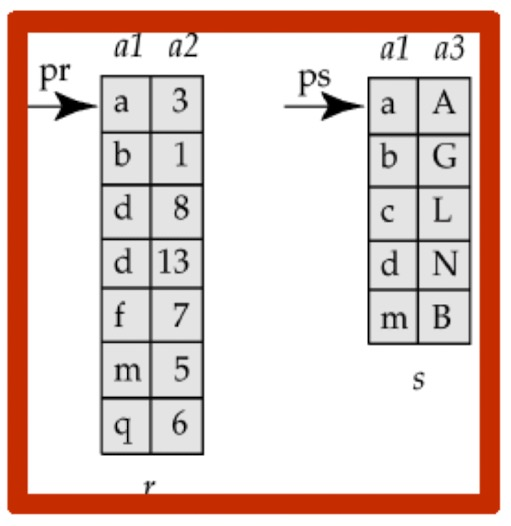
\includegraphics[width=\textwidth]{images/Screenshot 2024-05-25 at 11.56.19.jpg}
        \caption{Merge Join}
    \end{figure}
\end{minipage}
\begin{itemize}[label=\(\rhd\)]
    \item If all tuples for any given value of the join attributes fit in memory
    \begin{itemize}[label=\(\rhd\)]
        \item One file scan of $r$ and $s$ is enough
        \item $Cost = b_r + b_s$ (+ cost of sorting if relations are not sorted)
    \end{itemize}
    \item Otherwise, a block nested loop join must be performed between the tuples with the same attributes
    \item If the relation are not sorted appropriately we have to sort them. The combined operator is called a \textbf{sort-merge join}
\end{itemize}

\bigskip
\textbf{\underline{Hash Join}} \\

\begin{minipage}{0.5\textwidth}
\begin{itemize}[label=\(\rhd\)]
    \item Applicable for equi-joins and natural joins only
    \item Partition tuples of $r$ and $s$ using the \textbf{same} hash function $h$, which maps the values of the join attributes to the set $0,1,\cdots,n$
    \begin{itemize}[label=\(\rhd\)]
        \item Partitions of r-tuples: $r_0,r_1,\cdots,r_n$
        \begin{itemize}[label=\(\rhd\)]
            \item All $t_r \in r$ with $h(t_r[JoinAttrs])=i$ are put in $r_i$
        \end{itemize}
        \item Partitions of s-tuples: $s_0,s_1,\cdots, s_n$
        \begin{itemize}[label=\(\rhd\)]
            \item All $t_s \in s$ with $h(t_s[JoinAttrs])=i$ are put in $s_i$
        \end{itemize}
    \end{itemize}
    \item r-tuples in $r_i$ need only to be compared with s-tuples in $s_i$
    \begin{itemize}[label=\(\rhd\)]
        \item r-tuples and s-tuples that satisfy the join condition have the same hash value $i$, and are mapped to $r_i$ and $s_i$, respectively. 
    \end{itemize}
\end{itemize}
\end{minipage}
\hfill
\begin{minipage}{0.45\textwidth}
    \begin{figure}[H]
        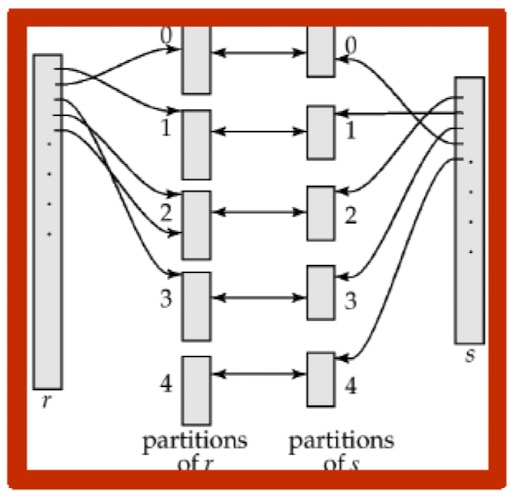
\includegraphics[width=\textwidth]{images/Screenshot 2024-05-25 at 11.50.16.jpg}
        \caption{Hash Join}
    \end{figure}
\end{minipage}
\begin{itemize}[label=\(\rhd\)]
    \item \textbf{Algorithm} for the hash join of $r$ and $s$
    \begin{enumerate}
        \item Partition the relation $s$ using hash function $h$. (When partitioning a relation, one block of memory is reserved as the output buffer for each relation)
        \item Partition $r$ similarly
        \item For each $i$:
        \begin{enumerate}[label*=\arabic*.] 
            \item Load $s_i$ into memory and \textbf{build} an in-memory hash index on it using the join attribute. This hash index uses a \textbf{different} hash function that the earlier one $h$
            \item Read the tuples in $r_i$ from the disk (block by block). For each tuple $t_r$ \textbf{probe} (locate) each matching tuple $t_s$ in $s_i$ using the in-memory hash index. Output the concatenation of their attributes as result tuple
        \end{enumerate}
    \end{enumerate}
    \item Relation $s$ is called the \textbf{build input} and $r$ is called the \textbf{probe input}
    \item \textbf{Cost analysis} of hash join
    \begin{itemize}[label=\(\rhd\)]
        \item Partitioning of the two relations: $2\cdot (b_r+b_s)$
        \begin{itemize}[label=\(\rhd\)]
            \item Complete reading of the two relations plus writing back
        \end{itemize}
        \item The build and probe phases read each of the partitions once: $b_r+b_s$
        \item $Cost=3\cdot(b_r+b_s)$
    \end{itemize}
\end{itemize}

\subsection{Query Optimization}
\begin{itemize}[label=\(\rhd\)]
    \item Alternatuve ways of evaluating a query because of 
    \begin{itemize}[label=\(\rhd\)]
        \item Equivalent expressions
        \item Different algorithms for each operation 
    \end{itemize}
    \item A \textbf{query evaluation plan} (query plan) is an annotated RA expression that specifies for each operator how to evaluate it 
    \item The cost difference between a good and a bad query evaluation plan can be enormous 
    \item The query optimizer needs to estimate the cost of operations
    \begin{itemize}[label=\(\rhd\)]
        \item Depends critically on statistical information about relations
        \item Estimates statistics for intermediate results to compute cost of complex expressions
    \end{itemize}
\end{itemize}

\bigskip
\textbf{\underline{Query Optimization}}\\

\begin{itemize}[label=\(\rhd\)]
    \item \textbf{Step 1: Parsing and translation}
    \begin{itemize}[label=\(\rhd\)]
        \item Translate the query into its internal form (query tree)
        \item The query tree corresponds to a \textbf{relational algebra (RA)} expression
        \item Each RA expression can be written as a \textbf{tree} where the algebra operator is the root and the argument relations are the children
    \end{itemize}
    \item \textbf{Step 2: Optimization}
    \begin{itemize}[label=\(\rhd\)]
        \item An RA expression may have many (semantically) equivalent expressions
        \item Each RA operation can be evaluated using one of several different algorithms
        \item \textbf{Evaluation plan}: Annotated RA expression that specifies for each operator detailed instructions on how to evaluate it
        \begin{itemize}[label=\(\rhd\)]
            \item like which index to use
        \end{itemize}
        \item \textbf{Goal of query optimization}: Among all equivalent evaluation plans choose the one with the lowest cost
    \end{itemize}
    \item \textbf{Step 3: Evaluation}
    \begin{itemize}[label=\(\rhd\)]
        \item The query-execution engine takes an evaluation plan, executes that plan, and returns the answers
    \end{itemize}
\end{itemize}

\textbf{Cost-based} optimization:
\begin{enumerate}
    \item Generate logically equivalent expressions by using equivalence rules to rewrite an expression into an equivalent one
    \item Annotate resulting expressions with information about algorithms/indexes for each operator
    \item Choose the cheapest plan based on \textbf{estimated cost}
\end{enumerate}
\textbf{Rule-based/heuristic} optimization:
\begin{enumerate}
    \item Generate logically equivalent expressions, controlled by a set of heuristic query optimization rules
\end{enumerate}

\subsubsection{Statistical Information}
\begin{itemize}[label=\(\rhd\)]
    \item $n_r$: number of tuples in relation $r$
    \item $b_r$: number of blocks containing tuples of $r$
    \item $s_r$: size of a tuple of $r$
    \item $f_r$: blocking factor of $r$, i.e., the number of tuples of $r$ that fit into one block
    \item $V(A,r)$: number of distinct values that appear in $r$ for attribute $A$; same as the size of $\pi_a(r)$
    \item $SC(A,r)$: selection cardinality of attribute $A$ of relation $r$; average number of records that satisfy equality on $A$
    \item $f_i$: average fan-out of internal nodes of index $i$
    \item $HT_i$: number of level in index $i$, i.e., the height of $i$
\end{itemize}

\subsubsection{Equivalence Rules}
$E,E_1,\cdots = $ RA expressions\\
$\theta,\theta_1,\cdots =$ predicates/conditions

\begin{itemize}[label=\(\rhd\)]
    \item \textbf{ER1} Conjunctive selection operations can be deconstructed into a sequence of individual selections\[
    \sigma_{\theta_1 \land \theta_2}(E) = \sigma_{\theta_1}(\sigma_{\theta_2}(E))
    \]
        \item \textbf{ER2} Selection operations are commutative \[
   \sigma_{\theta_1}(\sigma_{\theta_2}(E)) = \sigma_{\theta_2}(\sigma_{\theta_1}(E))
    \]
    \item \textbf{ER3} Only the last in a sequence of projections is needed, the others can be omitted ($L_i$ are lists of attributes) \[
    \pi_{L_1}(\pi_{L_2}(\cdots(\pi_{L_n}(E)) \cdots ))= \pi_{L_1}(E)
    \]
    \item \textbf{ER4} Selections can be combined with Cartesian product and theta joins
    \begin{itemize}[label=\(\rhd\)]
        \item[(a)] $\sigma_\theta(E_1 \times E_2) = E_1 \bowtie_\theta E_2$
        \item[(b)] $\sigma_{\theta_1}(E_1 \bowtie_{\theta_2}E_2)=E_1 \bowtie_{\theta_1 \land \theta_2} E_2$
    \end{itemize}
    \item \textbf{ER5} Theta joins (and natural joins) are commutative\[
    E_1 \bowtie_\theta E_2 = E_2 \bowtie_\theta E_1
    \]
    \item \textbf{ER6} Associativity
    \begin{itemize}[label=\(\rhd\)]
        \item[(a)] Natural join operations are associative: \[
        (E_1 \bowtie E_2) \bowtie E_3 = E_1 \bowtie (E_2\bowtie E_3)
        \]
        \item[(b)] Theta joins are associative in the following way:\[
        (E_1 \bowtie_{\theta_1}E_2) \bowtie_{\theta_2 \land \theta_3}E_3 = E_1 \bowtie_{\theta_1 \land \theta_3} (E_2 \bowtie_{\theta_2} E_3)
        \]
        where $\theta_2$ involves attributes from only $E_2$ and $E_3$
        \item[] Any of these conditions might be empty, hence, the Cartesian product operation is also associative
    \end{itemize}
    \item \textbf{ER7} The selection operation distributes over the theta join operation under the following conditions:
    \begin{itemize}[label=\(\rhd\)]
        \item[(a)] When all attributes in $\theta_o$ involve only the attributes of one of the expressions ($E_1$) being joined: \[
        \sigma_{\theta_o}(E_1 \bowtie_\theta E_2) = \sigma_{\theta_o}(E_1) \bowtie_\theta E_2
        \]
        \item[(b)] When $\theta_1$ involves only the attributes of $E_1$ and $\theta_2$ involves only the attributes of $E_2$: \[
        \sigma_{\theta_1 \land \theta_2}(E_1 \bowtie_\theta E_2) = \sigma_{\theta_1}(E_1) \bowtie_\theta \sigma_{\theta_2}(E_2)
        \] 
    \end{itemize}
    \item \textbf{ER8} The projection operation distributes over the theta join operation as follows:
    \begin{itemize}[label=\(\rhd\)]
        \item Let $L_1$ and $_2$ be sets of attributes from $E_1$ and $E_2$, respectively
        \item[(a)] if $\theta$ involves only attributes from $L_1 \cup L_2$:\[
        \pi_{L-1\cup L_2}(E_1 \bowtie_\theta E_2) = \pi_{L_1}(E_1) \bowtie_\theta \pi_{L_2}(E_2)
        \]
        \item[(b)] Consider a join $E_1 \bowtie_\theta E_2$
        \begin{itemize}[label=\(\rhd\)]
            \item Let $L_3$ be attributes of $E_1$ that are involved in join condition $\theta$, but are not in $L_1 \cup L_2$, and 
            \item Let $L_4$ be attributes of $E_2$ that are involved in join condition $\theta$, but are not in $L_1 \cup L_2$, and \[
            \pi_{L_1 \cup L_2}(E_1 \bowtie E_2) = \pi_{L_1 \cup L_2}(\pi_{L_1 \cup L_3}(E_1)\bowtie_\theta \pi_{L_2 \cup L_4}(E_2))
            \]
        \end{itemize}
    \end{itemize} 
    \item \textbf{ER9} The set operations union and intersection are commutative
    \begin{align*}
        E_1 \cup E_2 &= E_2 \cup E_1\\
        E_1 \cap E_2 &= E_2 \cap E_1
    \end{align*}
    \begin{itemize}[label=\(\rhd\)]
        \item[] Set difference is not commutative
    \end{itemize}
    \item \textbf{ER10} Set union and intersection are associative
    \begin{align*}
        (E_1 \cup E_2)\cup E_3 &= E_1 \cup (E_2\cup E_3)\\
        (E_1 \cap E_2) \cap E_3 &= E_1 \cap (E_2\cap E_3)
    \end{align*}
    \item \textbf{ER11} The selection operation distributes over $\cup, \cap$ and $-$ 
    \begin{align*}
        \sigma_\theta(E_1-E_2)&=\sigma_\theta(E_1)-\sigma_\theta(E_2) \\
        \sigma_\theta(E_1\cup E_2)&=\sigma_\theta(E_1)\cup \sigma_\theta(E_2) \\
        \sigma_\theta(E_1\cap E_2)&=\sigma_\theta(E_1)\cap \sigma_\theta(E_2)
    \end{align*}
    \item[] Also \begin{align*}
        &\sigma_\theta(E_1-E_2)=\sigma_\theta(E_1)-E_2 \\
        &\text{and similarly for $\cap$ in place of $-$, but not for $\cup$ }
    \end{align*} 
    \item \textbf{ER12} The projection operation distributes over union \[
    \pi_L(E_1\cup E_2)=\pi_L(E)\cup \pi_L(E_2)
    \]
\end{itemize}


\subsubsection{Heuristic Optimization}
\begin{itemize}[label=\(\rhd\)]
    \item Heuristic optimization transforms the query-tree by using a set of heuristic rules that typically (but not in all cases) improve execution performance
    \item Overall goal of heuristic rules:
    \begin{itemize}[label=\(\rhd\)]
        \item Try to \textbf{reduce the size of (intermediate) relations} as early as possible
    \end{itemize}
    \item Heuristic rules:
    \begin{itemize}[label=\(\rhd\)]
        \item Perform selection early
        \item Perform projection early
        \item Perform most restrictive selection and join operations before other similar operations
    \end{itemize}
    \item Steps in typical heuristic optimization
    \begin{enumerate}
        \item Break up conjunctive selections into a sequence of single selection operations (\textbf{ER1})
        \item Move selection operations down the query tree for the earliest possible execution (\textbf{ER2, ER7}(a), \textbf{ER7}(b), \textbf{ER11})
        \item Execute first those selection and join operations that will produce the smallest relations (\textbf{ER6})
        \item Replace Cartesian product operations that are followed by a selection condition by join operations (\textbf{ER4}(a))
        \item Deconstruct and move as far down the tree as possible lists of projection attributes, creating new projections where needed (\textbf{ER3, ER8}(a), \textbf{ER8}(b), \textbf{ER12})
        \item Identify those subtrees whose operations can be pipelined, and execute them using pipelining
    \end{enumerate}
\end{itemize}

\subsubsection{Cost-Based Optimization}
Basic working of a cost-based query optimizer:
\begin{itemize}[label=\(\rhd\)]
    \item \textbf{Algorithm}
    \begin{enumerate}
        \item Use transformations (equivalence rules) to generate multiple candidate evaluation plans from the original evaluation plan.
        \item Cost formulas estimate the cost of executing each operation in each candidate evaluation plan
        \begin{itemize}[label=\(\rhd\)]
            \item Cost formulas are parameterized by
            \begin{itemize}[label=\(\rhd\)]
                \item statistics of the input relations;
                \item dependent on the specific algorithm used by the operator;
                \item CPU time, I/O time, communication time, main memory usage, or a combination
            \end{itemize}
        \end{itemize}
        \item The candidate evaluation plan with the \textbf{least total cost} is selected for execution
    \end{enumerate}
\end{itemize}

\subsubsection{Example}
Consider a DB with the following characteristics:
\begin{itemize}[label=\(\rhd\)]
    \item $|r_1(A,B,C)|=1000,\ V(C,r_1) = 900$
    \item $|r_2(C,D,E)|=1500,\ V(C,r_2) = 1100,\ V(E,r_2)=50$
    \item $|r_3(E,F)|=750,\ V(E,r_3)=100$
\end{itemize}
Estimate the size of $r_1 \bowtie r_2 \bowtie r_3$ and determine an efficient evaluation strategy.
\begin{align*}
    |r_1 \bowtie r_2| &= |r_1| \cdot \frac{|r_2|}{V(C,r_2)} &&= 1364 \\
    |r_2 \bowtie r_1|&= |r_2| \cdot \frac{|r_1|}{V(C,r_1)} &&= 1667\\
    |r_3 \bowtie r_1| &= 750'000 &&\text{Cartesian Prod. (no join condition)}\\
    |r_3 \bowtie r_2| &= 750 \cdot \frac{1500}{50} &&= 22'500 \\
    |r_2 \bowtie r_3| &= 11'250 \\
    |(r_1 \bowtie r_2) \bowtie r_3| &= |r_1 \bowtie r_2| \cdot \frac{|r_3|}{V(E,r_3)} &&= 10'230 \\
    |r_1 \bowtie (r_2 \bowtie r_3)| &= |r_1| \cdot \frac{|r_2 \bowtie r_3|}{V(C, r_{23})} &&= 10'227 \quad \text{guess $\approx V(C,r_2)$ for $V(C,r_{2,3})$}\\
    |(r_2 \bowtie r_3) \bowtie r_1| &= 11'250 \cdot \frac{100}{900} &&= 12'500
\end{align*}


\subsection{Summary}
\begin{itemize}[label=\(\rhd\)]
    \item Query evaluation techniques:
    \begin{itemize}[label=\(\rhd\)]
        \item Physical sorting:
        \begin{itemize}[label=\(\rhd\)]
            \item Physical sorting is a basic and important technique
            \item The same sort order should be useful to many operators and not just one (global vs, local optimization)
        \end{itemize}
        \item Evaluation techniques for selections:
        \begin{itemize}[label=\(\rhd\)]
            \item Use primary index if available; secondary index is much worse
            \item Equality conditions are selective and should be optimized 
            \item Linear scan with sequential IO is the base line for selections
        \end{itemize}
        \item Evaluation techniques for joins:
        \begin{itemize}[label=\(\rhd\)]
            \item Nested loop: base line; avoid whenever possible 
            \item Sort merge: robust and fast
            \item Hash join: fastest; only for equality
        \end{itemize}
    \end{itemize}
    \item Query optimization techniques
    \begin{itemize}[label=\(\rhd\)]
        \item \textbf{Equivalence rules} for relational algebra expressions (must holds for multisets)
        \item \textbf{Rule-based query optimization} is based on heuristics (usually the goal is to keep intermediate results as small as possible)
        \item \textbf{Cost-based query optimization} uses statistical information to find the cheapest (or reasonably cheap) plan
    \end{itemize}
\end{itemize}